\section{Método de solución}

Consideraremos una estructura de \(n\) pisos, la cual se puede modelar mediante \eqref{eqn:final-matrix-form}. Además, consideraremos que la estructura parte del reposo y de la posición de equilibrio. Esto nos aporta las condiciones iniciales \(\mathbf{u}(0) = \mathbf{0}\) y \(\mathbf{u}'(0) = \mathbf{0}\).

\subsection{Intento utilizando transformada de Laplace}

Podemos considerar el problema reducido de las ecuaciones para una estructura de \(n = 2\) pisos bajo los siguientes parámetros simplificados:
\begin{gather}
    m_1 = m_2 = m \\
    c_2 = 0, \, c_1 = c \\
    k_1 = k_2 = k \\
    \mathbf{u}(0) = \mathbf{u}'(0) = \mathbf{0} \\
    P_1(t) = A\sin(\omega t), \, P_2(t) = 0
.\end{gather}

Entonces, la ecuación sería
\[
    \begin{bmatrix}
        m & 0 \\
        0 & m
    \end{bmatrix} \begin{bmatrix} u_1'' \\ u_2'' \end{bmatrix}
    + \begin{bmatrix}
        c & 0 \\
        0 & 0
    \end{bmatrix} \begin{bmatrix} u_1' \\ u_2' \end{bmatrix}
    + \begin{bmatrix}
        2k & -k \\
        -k & k
    \end{bmatrix} \begin{bmatrix} u_1 \\ u_2 \end{bmatrix}
    = \begin{bmatrix} A\sin(\omega t) \\ 0 \end{bmatrix}
,\]
la cual se puede expresar como el sistema
\[
    \begin{cases}
        mu_1'' + cu_1' + 2ku_1 - ku_2 = A\sin(\omega t) \\
        mu_2'' - ku_1 + ku_2 = 0
    .\end{cases}
\]

Aplicando la transformada de Laplace a ambos lados de la ecuación, obtenemos
\[
    \begin{cases}
        m\mathcal{L}\{u_1''\} + c\mathcal{L}\{u_1'\} + 2k\mathcal{L}\{u_1\} - k\mathcal{L}\{u_2\} = A\mathcal{L}\{\sin(\omega t)\} \\
        m\mathcal{L}\{u_2''\} - k\mathcal{L}\{u_1\} + k\mathcal{L}\{u_2\}= 0
    .\end{cases}
\]

Aplicando las condiciones iniciales \(u_1(0) = u_2(0) = u_1'(0) = u_2'(0) = 0\) para aprovechar las propiedades de la transformada de Laplace de la derivada de una función, la ecuación toma la siguiente forma:
\[
    \begin{cases}
        ms^2\mathcal{L}\{u_1\} + cs\mathcal{L}\{u_1\} + 2k\mathcal{L}\{u_1\} - k\mathcal{L}\{u_2\} = \frac{A\omega}{s^2+\omega^2} \\
        ms^2\mathcal{L}\{u_2\} - k\mathcal{L}\{u_1\} + k\mathcal{L}\{u_2\}= 0
    .\end{cases}
\]

Factorizando y reescribiendo, el sistema nos queda
\[
    \begin{cases}
        (ms^2+cs+2k)\mathcal{L}\{u_1\} - k\mathcal{L}\{u_2\} = \frac{A\omega}{s^2+\omega^2} \\
        - k\mathcal{L}\{u_1\} + (ms^2+k)\mathcal{L}\{u_2\} = 0
    .\end{cases}
\]
lo cual, en forma matricial, es lo mismo que
\[
    \begin{bmatrix}
        ms^2+cs+2k & -k \\
        -k & ms^2+k
    \end{bmatrix} \begin{bmatrix} \mathcal{L}\{u_1\} \\ \mathcal{L}\{u_2\} \end{bmatrix}
    = \begin{bmatrix} \frac{A\omega}{s^2+\omega^2} \\ 0 \end{bmatrix}
.\]

Para hallar las funciones \(u_1\) y \(u_2\), necesitamos despejar el sistema de ecuaciones en términos de la transformada de Laplace de ambas funciones. Para realizar esto, usamos la regla de Cramer. Empezamos calculando el determinante de la matriz de coeficientes:
\[
    \Delta = \begin{vmatrix}
        ms^2+cs+2k & -k \\
        -k & ms^2+k
    \end{vmatrix} = m^2s^4+mcs^3+3mks^2+cks+k^2.
\]

Obteniendo las expresiones para \(\mathcal{L}\{u_1\}\) y \(\mathcal{L}\{u_2\}\):
\[
    \mathcal{L}\{u_1\} =
    \frac{1}{\Delta} \begin{vmatrix}
        \frac{A\omega}{s^2+\omega^2} & -k \\
        0 & ms^2+k
    \end{vmatrix}
    = \frac{A\omega ms^2+A\omega k}{(m^2s^4+mcs^3+3mks^2+cks+k^2)(s^2+\omega^2)}
,\]
\[
    \mathcal{L}\{u_2\} =
    \frac{1}{\Delta} \begin{vmatrix}
        ms^2 + cs + 2k & \frac{A\omega}{s^2 + \omega^2} \\
        -k & 0
    \end{vmatrix}
    = \frac{A\omega k}{(m^2s^4+mcs^3+3mks^2+cks+k^2)(s^2+\omega^2)}
.\]

Por lo tanto, el nuevo sistema nos queda
\[
    \begin{cases}
        \mathcal{L}\{u_1\} = \frac{A\omega ms^2+A\omega k}{(m^2s^4+mcs^3+3mks^2+cks+k^2)(s^2+\omega^2)} \\
        \mathcal{L}\{u_2\} = \frac{A\omega k}{(m^2s^4+mcs^3+3mks^2+cks+k^2)(s^2+\omega^2)}.
    .\end{cases}
\]

Aplicando la transformada inversa de Laplace, tenemos
\[
    \begin{cases}
        u_1 = \mathcal{L}^{-1}\{\frac{A\omega ms^2+A\omega k}{(m^2s^4+mcs^3+3mks^2+cks+k^2)(s^2+\omega^2)}\} \\
        u_2 = \mathcal{L}^{-1}\{\frac{A\omega k}{(m^2s^4+mcs^3+3mks^2+cks+k^2)(s^2+\omega^2)}\}
    .\end{cases}
\]

Aunque, en teoría, se puede encontrar una solución explícita utilizando métodos computacionales como MATLAB para aplicar la transformada inversa, estas soluciones son extremadamente extensas. Incluso reemplazando los parámetros realistas presentados en \eqref{eqn:sol-sismo-params} (cuyo origen se detallará más adelante), y aplicando la inversa en MATLAB, se obtienen resultados que involucran números en los órdenes alrededor de \(10^{77}\). Esto no significa que la solución en sí esté en tales órdenes, pero las expresiones sí involucran tales cantidades.

Claramente, utilizar métodos analíticos para resolver estas ecuaciones no parece producir resultados cómodos de usar. Computacionalmente, trabajar con números de tales órdenes es extremadamente ineficiente. Por lo tanto, a continuación resolveremos las ecuaciones utilizando métodos numéricos.


\subsection{Utilizando métodos numéricos}

Para resolver este sistema con las condiciones iniciales dadas, utilizaremos el método de Runge-Kutta de orden 4 (RK4), el cual se detalla en el marco teórico del informe. Sin embargo, para ello será necesario llevar \eqref{eqn:final-matrix-form} a la forma
\[
    \mathbf{x}' = \mathbf{f}(t, \mathbf{x})
.\]

Para ello, podemos definir \(\mathbf{v} = \mathbf{u}'\), lo cual transforma \eqref{eqn:final-matrix-form} (un sistema de \(n\) ecuaciones) en el siguiente sistema de \textit{primer orden} de \(2n\) ecuaciones:

\[
    \begin{cases}
        \mathbf{v} = \mathbf{u}' \\
        M\mathbf{v}' + C\mathbf{v} + K\mathbf{u} = \mathbf{P}(t)
    .\end{cases}
\]

Nótese que cada una de estas ecuaciones matriciales aporta \(n\) ecuaciones al sistema.

Para aplicar el método de RK4 a este sistema, lo colocaremos en la forma
\begin{equation}\label{eqn:substituted-system}
    \begin{cases}
        \mathbf{u}' = \mathbf{v} \\
        \mathbf{v}' = M^{-1}(-C\mathbf{v} - K\mathbf{u} + \mathbf{P}(t))
    .\end{cases}
\end{equation}

Nótese también que \(M^{-1}\) siempre existe (y es trivial) puesto que \(M\) es una matriz diagonal cuyos elementos en dicha diagonal son todos no-nulos:
\[
    M^{-1} = \begin{bmatrix}
        1/m_1 & 0 & \cdots & 0 \\
        0 & 1/m_2 & \cdots & 0 \\
        \vdots & \vdots & \ddots & \vdots \\
        0 & 0 & \cdots & 1/m_n
    \end{bmatrix}
.\]

Ahora podemos expresar \eqref{eqn:substituted-system} mediante una sola ecuación matricial con \(\mathbf{u}\) y \(\mathbf{v}\) concatenados en un solo vector \(\mathbf{x}\) como
\begin{equation}\label{eqn:rk4-ready}
    \mathbf{x}' = \mathbf{f}(t, \mathbf{x})
,\end{equation}
donde definimos
\[
    \mathbf{x} = \begin{bmatrix} \mathbf{u} \\ \mathbf{v} \end{bmatrix}_{2n \times 1},
    \qquad
    \mathbf{f}(t, \mathbf{x}) = \mathbf{f}\left(t, \begin{bmatrix} \mathbf{u}_{n \times 1} \\ \mathbf{v}_{n \times 1} \end{bmatrix}\right) = \begin{bmatrix}
        \mathbf{v} \\
        M^{-1}(-C\mathbf{v} - K\mathbf{u} + \mathbf{P}(t))
    \end{bmatrix}_{2n \times 1}
.\]

Nótese que las condiciones iniciales que establecimos (\(\mathbf{u}(0) = \mathbf{u}'(0) = \mathbf{v}(0) = \mathbf{0}\)) producen en conjunto la condición \(\mathbf{x}(0) = \mathbf{0}\). Además, trabajaremos RK4 con el tiempo inicial \(t_0 = 0\).

Entonces, el procedimiento que usaremos será el siguiente:

\begin{enumerate}
    \item Definir un tiempo final \(t_s\) y una cantidad \(s\) de pasos.
    \item Calcular el avance por iteración: \(h = \frac{t_s - t_0}{s}\).
    \item Aplicar el método de RK4 para sistemas de EDOs explicado en el apéndice~\ref{appendix:rk4-systems}.
\end{enumerate}

Al final del proceso, los valores de \(\mathbf{x}\) obtenidos contendrán en sus primeras mitades los puntos calculados para las posiciones \(u_1, u_2, \ldots, u_n\) de los pisos a través del tiempo. Sus segundas mitades contendrán los valores de las derivadas \(u_1', u_2', \ldots, u_n'\), pero estas no se graficarán.

Nótese que, en lugar de definir explícitamente un valor para el avance \(h\), definimos un \textit{tiempo final} \(t_s\) y calculamos \(h\) en función de este y la cantidad de pasos deseada, puesto que resulta más conveniente definir un tiempo de llegada y una cantidad de pasos que denoten la ``precisión'' a utilizar.

Los resultados presentados a continuación fueron obtenidos con una precisión de \(s = 10,000\) pasos.

\subsubsection*{Resultados para parámetros particulares}

Se presentan a continuación las gráficas resultantes para ciertos conjuntos de parámetros particulares. La implementación en Python de RK4 usada se encuentra en el apéndice~\ref{appendix:rk4-code}.

Los valores de masa, amortiguamiento y elasticidad que utilizaremos se basan en el trabajo de \citet{tarque}, quienes presentan los siguientes parámetros para un edificio de tres pisos de un estudio real:
\begin{gather}\label{eqn:sol-sismo-params}
    m_1 = m_2 = m_3 = 150 \, \si{ton} = 150,000 \, \si{kg}, \\
    k_1 = k_2 = k_3 = 200,000 \, \si{N/m}, \\
    \zeta_1 = 5\%, \quad \zeta_2 = \zeta_3 = 0\%
,\end{gather}
de donde (como se explicó en el marco teórico sobre las razones de amortiguamiento) se obtienen los coeficientes de amortiguamiento \(c_1 = 5\%(2\sqrt{m_1 k_1}) \approx 16,497.13 \, \si{kg/s}, \,
c_2 = c_3 = 0 \, \si{kg/s}\). Aunque se tratan de parámetros para un edificio, estos parámetros son de igual manera una referencia válida para parámetros de un puente de 3 pisos.


% En primer lugar, podemos considerar una fuerza externa nula \(\mathbf{P}(t) = \mathbf{0}\). La figura~\ref{fig:sol-p-0} muestra que, como es de esperarse, ninguno de los pisos presenta movimiento alguno.
%
% \begin{figure}[ht!]
%     \centering
%     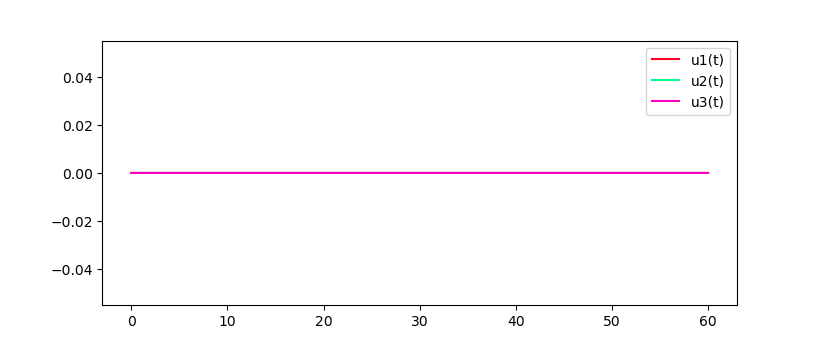
\includegraphics[width=\textwidth]{sol_p_0}
%     \caption{Gráfica de \(\mathbf{u}(t)\) con \(\mathbf{P}(t) = \mathbf{0}\) para \(t \in [0, 60]\)}
%     \label{fig:sol-p-0}
% \end{figure}

Consideramos una fuerza externa de la forma \(P_1(t) = m_1 a_g(t)\) ejercida sobre el primer piso. Esta tipo de función se utiliza para representar la fuerza ejercida sobre la base de una estructura durante un sismo \citep{kramer}, donde \(a_g(t)\) es la aceleración del suelo en función del tiempo. En particular, tomaremos \(a_g\) como una sinusoidal de la forma \(a_g(t) = A\sin(2\pi f t)\), donde \(A\) (en \(\si{m/s^2}\)) es la aceleración pico del suelo y \(f\) (en \(\si{Hz}\)) es su frecuencia de oscilación. En particular, tomaremos una aceleración pico de \(A = 0.3 \, \si{m/s^2}\) y frecuencia de oscilación de \(f = 4 \, \si{Hz}\)

Experimentaremos a continuación con estos parámetros y variaciones de ellos. Cabe destacar que todas las gráficas usarán segundos para el tiempo \(t\) y metros para los desplazamientos \(u_1, u_2, \ldots, u_n\).

Con los parámetros especificados anteriormente obtenemos la figura~\ref{fig:sol-sismo-corto}. Sin embargo, se puede apreciar mejor el comportamiento a largo plazo de las vibraciones si extendemos la gráfica hasta un tiempo de 180 segundos (véase la figura~\ref{fig:sol-sismo-largo}).


\begin{figure}[ht!]
    \centering
    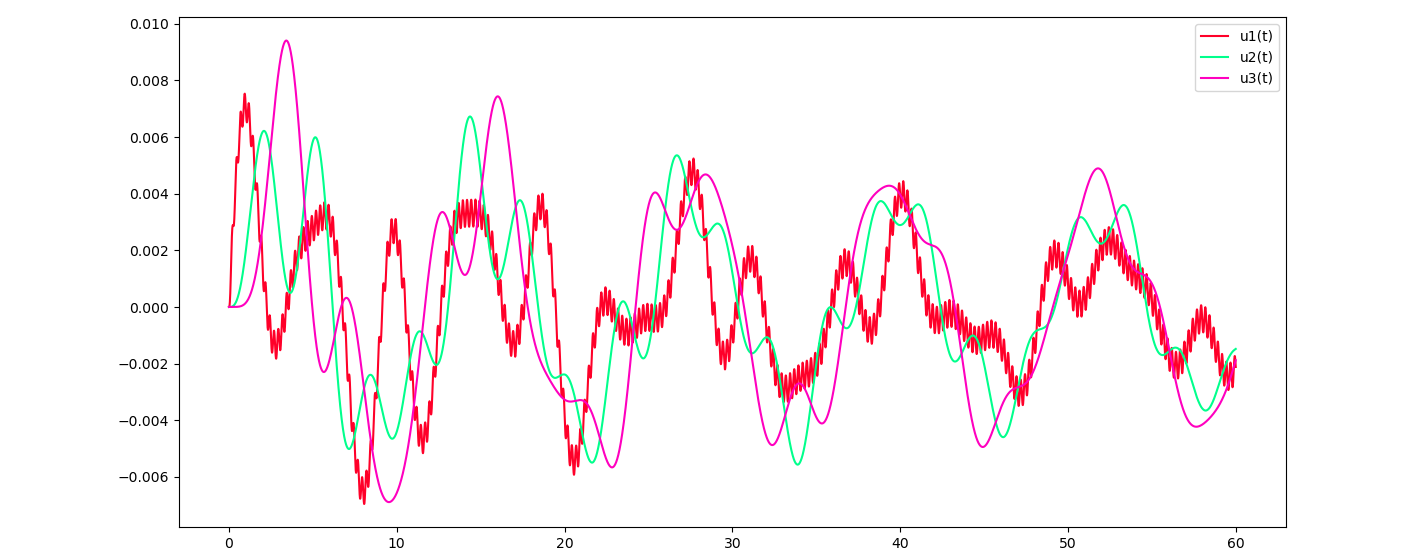
\includegraphics[width=\textwidth]{sol_sismo_corto}
    \caption{Gráfica de \(\mathbf{u}(t)\) con \(P_1(t) = m_1 A \sin(2\pi f t)\) para \(t \in [0, 60]\).}
    \label{fig:sol-sismo-corto}
\end{figure}

\begin{figure}[ht!]
    \centering
    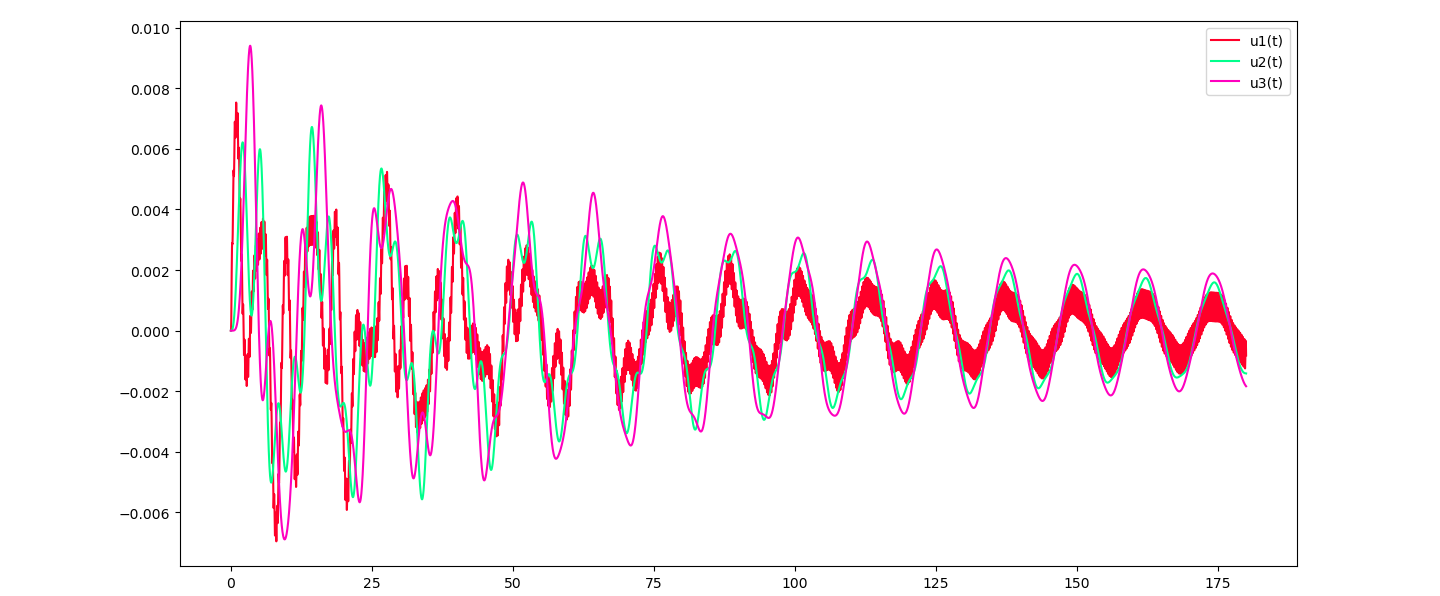
\includegraphics[width=\textwidth]{sol_sismo_largo}
    \caption{Gráfica de \(\mathbf{u}(t)\) con \(P_1(t) = m_1 A \sin(2\pi f t)\) para \(t \in [0, 180]\).}
    \label{fig:sol-sismo-largo}
\end{figure}

Si aumentamos las razones de amortiguamiento de \eqref{eqn:sol-sismo-params} a
\[
    \zeta_1 = 10\%, \quad \zeta_2 = 5\%, \quad \zeta_3 = 2.5\%
,\]
se produce la figura~\ref{fig:sol-sismo-damped}. En esta gráfica, se puede notar que la amplitud de las vibraciones de la estructura se reduce más rápidamente que en la figura~\ref{fig:sol-sismo-largo}.

\begin{figure}[ht!]
    \centering
    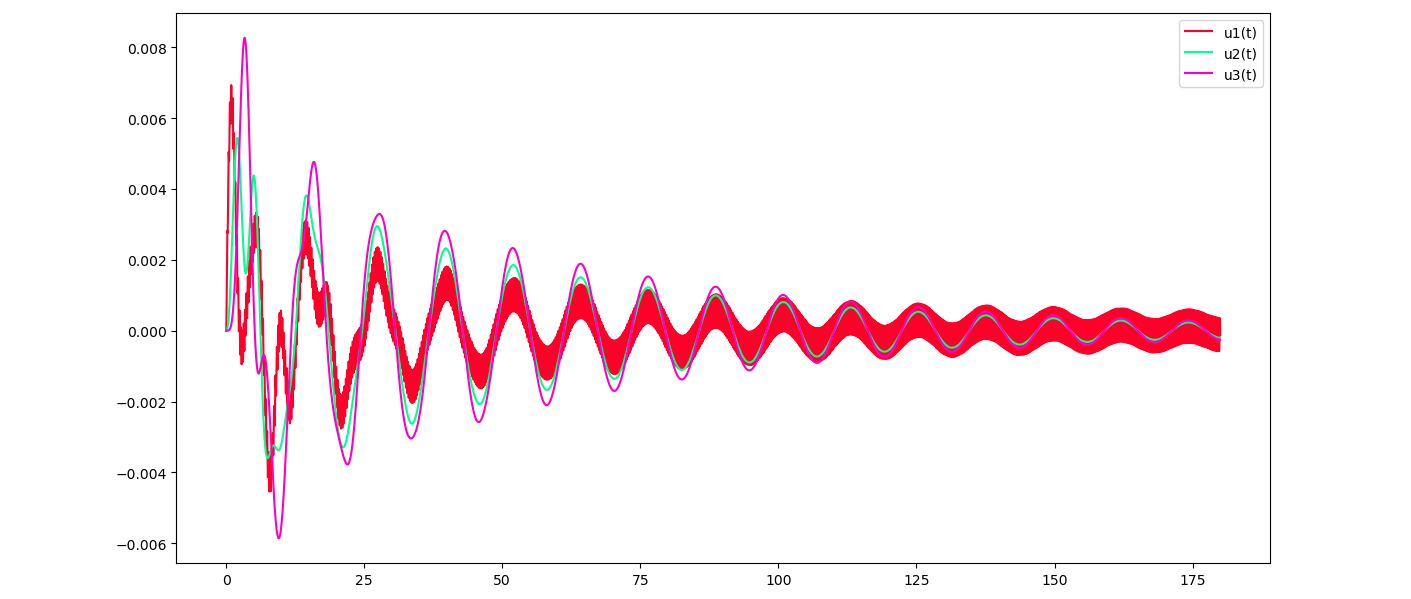
\includegraphics[width=\textwidth]{sol_sismo_damped}
    \caption{Gráfica de \(\mathbf{u}(t)\) con \(P_1(t) = m_1 A \sin(2\pi f t)\) para \(t \in [0, 180]\) (amortiguamiento aumentado).}
    \label{fig:sol-sismo-damped}
\end{figure}

Si, en lugar de aumentar el amortiguamiento, aumentamos los coeficientes elásticos de \eqref{eqn:sol-sismo-params} a
\[
    k_1 = 200,000 \, \si{N/m}, \quad k_2 = 500,000 \, \si{N/m}, \quad k_3 = 800,000 \, \si{N/m}
,\]
se obtiene la figura~\ref{fig:sol-sismo-elastic}.

\begin{figure}[ht!]
    \centering
    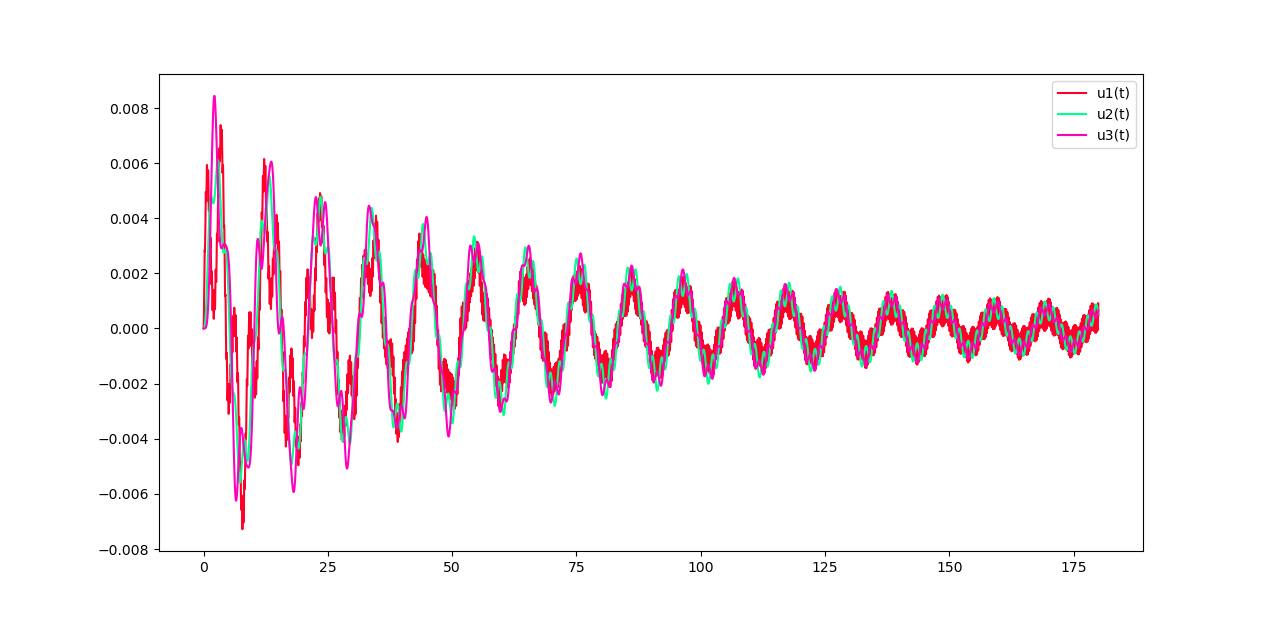
\includegraphics[width=\textwidth]{sol_sismo_elastic}
    \caption{Gráfica de \(\mathbf{u}(t)\) con \(P_1(t) = m_1 A \sin(2\pi f t)\) para \(t \in [0, 180]\) (elasticidad aumentada).}
    \label{fig:sol-sismo-elastic}
\end{figure}

A su vez, si tomamos los parámetros \eqref{eqn:sol-sismo-params} y duplicamos la masa del primer piso a \(m_1 = 300,000 \, \si{kg}\), se produce la figura~\ref{fig:sol-sismo-heavy}.

\begin{figure}[ht!]
    \centering
    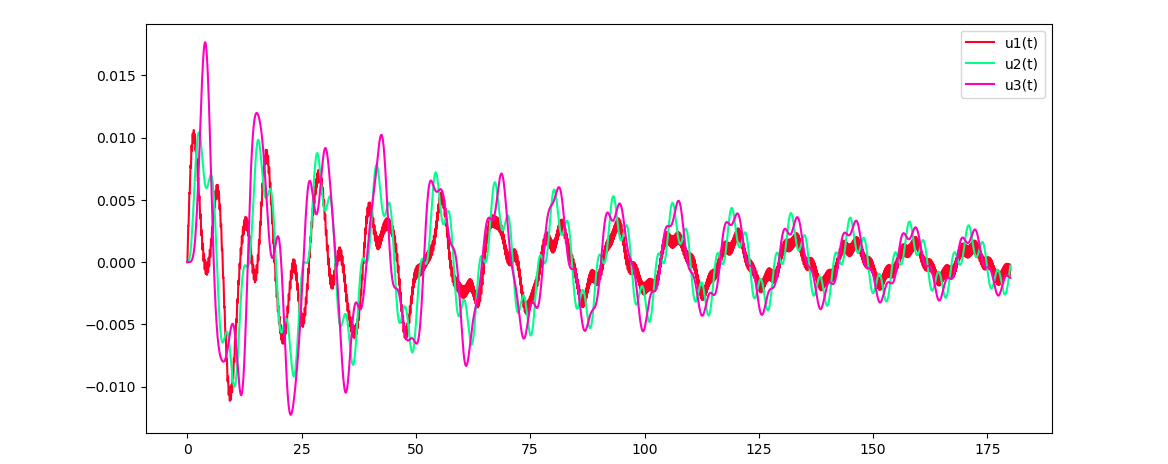
\includegraphics[width=\textwidth]{sol_sismo_heavy}
    \caption{Gráfica de \(\mathbf{u}(t)\) con \(P_1(t) = m_1 A \sin(2\pi f t)\) para \(t \in [0, 180]\) (masa del primer piso aumentada).}
    \label{fig:sol-sismo-heavy}
\end{figure}

Un fenómeno particularmente interesante ocurre cuando, usando los parámetros originales \eqref{eqn:sol-sismo-params}, cambiamos la frecuencia de \(P_1(t)\) a \(f = 0.0819 \, \si{Hz}\). Esta frecuencia, la cual se encuentra extremadamente cerca a la \textit{frecuencia natural} de la estructura  produce la figura~\ref{fig:sol-sismo-resonance}. Se incluye más información sobre este fenómeno y cómo se llegó a dicha frecuencia en el apéndice~\ref{appendix:natural-frequency}

\begin{figure}[ht!]
    \centering
    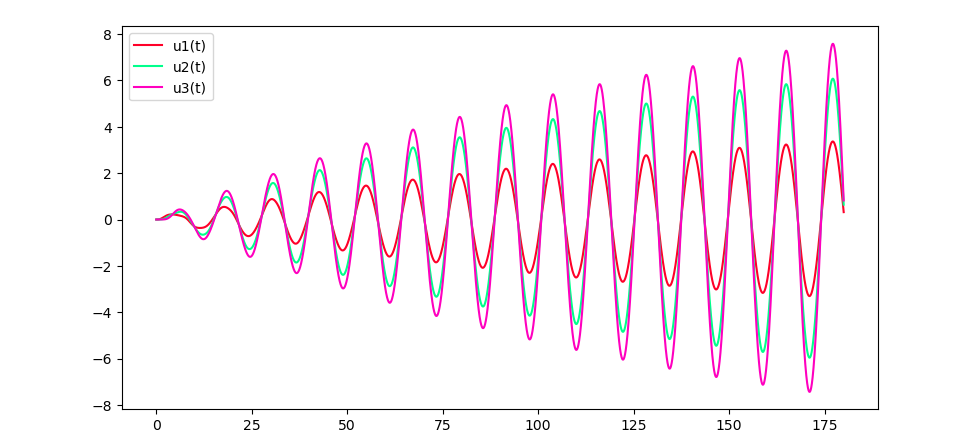
\includegraphics[width=\textwidth]{sol_sismo_resonance}
    \caption{Gráfica de \(\mathbf{u}(t)\) con \(P_1(t) = m_1 A \sin(2\pi f t)\) para \(t \in [0, 180]\) (en resonancia).}
    \label{fig:sol-sismo-resonance}
\end{figure}
